\documentclass[11pt,a4]{jarticle}
\usepackage[top=25truemm,bottom=30truemm,left=20truemm,right=20truemm]{geometry}
\usepackage{graphicx}
\usepackage{comment}
\begin{document}

\title{半導体の物性と基本的なデバイス応用}
\maketitle
\tableofcontents

\section{実験の目的}
本実験は半導体デバイスの振る舞いを確認しながら、その動作原理の理解を深めることを目的とする。
特に半導体の光応答や磁場下での振る舞いは、基礎物性の観点から、また応用やデバイス化の観点から極めて重要であるので掘り下げて勉強する。
また半導体の物性を測定するための基本的な実験手法を学ぶ。
\section{実験方法}

\subsection{ダイオード}
結晶中の電子の取りうるエネルギー準位は、有限のエネルギー範囲の中で連続的に分布しており、電子は低い準位から順番に占有する。この連続的なエネルギー準位をエネルギーバンドと呼ぶ。
エネルギーバンドの内部が電子で埋め尽くされているとき、そのエネルギーバンドは電気伝導に寄与しない。しかしエネルギーバンドの内部の一部のみを電子が占めているとき、もしくは一部に空いた準位が存在するとき、そのエネルギーバンドでは電気伝導現象が観測される。そのときの電気伝導の担い手(キャリア)をそれぞれ伝導電子と正孔という。伝導電子が存在するエネルギーバンドを伝導帯と呼び、伝導帯の低エネルギー側に隣接するエネルギーバンドを価電子帯と呼ぶ。伝導帯と価電子帯のエネルギー差をエネルギーギャップという。

正孔を多数キャリアとする半導体をp型半導体といい、伝導電子を多数キャリアとする半導体をn型半導体という。p型半導体とn型半導体を接合すると(pn接合)、以下に説明するように整流特性をもつ(図挿入)。
接合面周辺でn型半導体の電子はp型半導体に向かって拡散し、p型半導体の正孔はn型半導体に向けて拡散する。ここで電子と正孔の結合が起きるため、接合面ではキャリアが存在しない層ができる(空乏層)。この空乏層が整流効果をうむ。接合のp型半導体側を高電位とすると(順電圧)、そうでないときに比べ空乏層の幅は狭まり、電流は流れやすい。n型半導体側を高電位とすると(逆電圧)、そうでないときに比べ空乏層の幅は拡がり、電流は流れにくくなる。このときの電圧電流特性(V-J特性)を表したものが式\ref{eq:C1-30}である。ここで$q$は素電荷、Tは温度、$k_B$はボルツマン係数、$J_s$は電子と正孔び熱生成電流(短絡電流)である。
\begin{equation}
J / J_s = exp(qV/ k_B T)- 1
\label{eq:C1-30}
\end{equation}

以下に述べるように発光ダイオードやフォトダイオード、太陽電池は、pn接合面での整流特性を利用したデバイスである。空乏層に光が入射したとき価電子帯の電子の一部がバンドギャップより大きい光エネルギーを吸収すると、電子は伝導帯に励起される。すなわち伝導帯に電子が、価電子帯に正孔が生成しともに電気伝導に寄与する。このときダイオードに流れる電流は入射する光の量(例えばエネルギー)に依存する。これを用いたデバイスがフォトダイオードである。フォトダイオードは発電に用いることもできる。これを太陽電池と言う。
フォトダイオードとは逆のプロセスを考える。pn接合に電圧を印加すると、ある電圧以上で化学ポテンシャルより大きなエネルギーを持った光励起。このとき印加電圧が一定以上の大きさであることが必要である。この効果を利用したデバイスが発光ダイオードである。


\subsubsection{発光ダイオードの発光特性}
青色と緑色、赤色それぞれの発光ダイオードに印加する電圧を変化させて、肉眼で明るさを観察した。肉眼で発光が確認できる最小の印加電圧を記録した。

\subsubsection{フォトダイオードの電圧電流特性}
図\ref{fig:photodiode_setup}にフォトダイオードの電圧電流特性測定実験の回路図を示す。

まず発光ダイオードに電圧を印加せずに、発光ダイオードを発光させない条件で実験を行った。そのときのフォトダイオードに印加する電圧を順方向から逆方向まで変化させたときに、フォトダイオードに流れる電流を測定した。

そのあと発光ダイオードに電圧を印加し、その電圧を変化させながら、電圧を印加しない場合と同様にフォトダイオードの電圧電流特性の測定を行った。
\begin{figure}[!htbp]
   \begin{center}
    \includegraphics[width=0.8\hsize]{./photodiode_setup.eps}
    \caption{フォトダイオードの電圧電流特性測定回路}
     \label{fig:photodiode_setup}
   \end{center}
\end{figure}

\subsubsection{太陽電池の電圧電流特性}
フォトダイオードの電圧電流特性の測定実験と同様である。図\ref{fig:solor_cell_setup}に太陽電池の電圧電流特性実験のの回路図を示す。太陽電池に入射光源には白熱電球を用いて、その電球光源の電源を切ったときと、つけた時の太陽電池の電圧電流特性を測定した。
\begin{figure}[!htbp]
   \begin{center}
    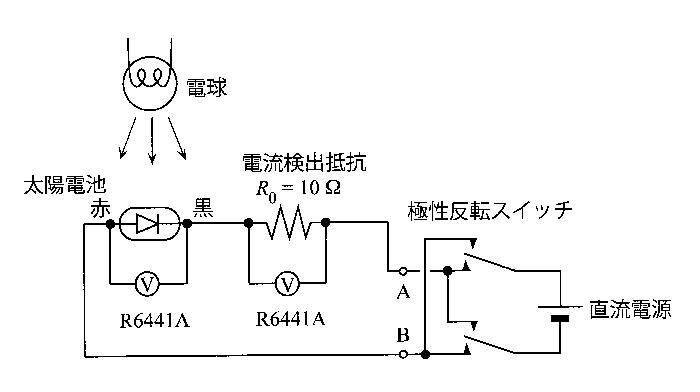
\includegraphics[width=0.7\hsize]{./solor_cell_setup.eps}
    \caption{太陽電池の電圧電流特性回路}
     \label{fig:solor_cell_setup}
   \end{center}
\end{figure}

\subsection{導電率とHall係数の測定}
電荷$q$を持つキャリアが密度$n$で半導体中に存在するとする。
キャリアの運動を説明するために、Drude-Sommerfeldのモデルを仮定する。すなわち平均速度$v$で移動するキャリア(有効質量$m$)は、統計的に見ると一定時間$\tau$ごとに散乱されるとする。このとき物質中の電場$E$と電流密度$j=nqv$は比例関係にある(オームの法則)。
\begin{equation} 
E = \sigma j
\label{eq:conductivity}
\end{equation}
ここで比例係数$\sigma$は導電率と呼ばれる。
また電磁場中でキャリアにLorentz力$F = qE + j \times B$が働く。

このとき導電率$\sigma$はキャリア濃度$n$と移動度$\mu=q\tau/m$によって次のように表される。
\begin{equation}
\sigma = n q \mu
\label{eq:sigma}
\end{equation}

定常状態で半導体内部のローレンツ力は0となる。流れる電流と磁場が直交しているとき、それらにさらに直交する方向にローレンツ力を打ち消す電場が励起される。これをHall電場と呼ぶ。Hall電場$E_{Hall}$は磁束密度$B$と電流密度に比例し、その比例係数$R_H$をHall係数と呼ぶ。この比例係数の符号から、主に伝導に寄与するキャリアの電荷の符号が分かる。ここでHall係数$R_H$はキャリア濃度によって次のように表される。
\begin{equation}
R_H = 1/ n q 
\label{eq:R_H}
\end{equation}

導電率$\sigma$に関する表式\ref{eq:sigma}と移動度に関する表式\ref{eq:R_H}から、導電率$\sigma$とHall係数$R_H$が求まると、キャリア濃度$n$と移動度$\mu$が求まる。


図に本実験に用いた試料の模式図を示す。電圧は1-2端子間に印加されて、磁場は紙面に対して垂直に印加される。このときの3-4端子間の電圧を計測することで導電率を計算し、5-6端子間の電圧を計測することでHall係数を計算する。
\begin{figure}[!htbp]
   \begin{center}
    \includegraphics[width=0.5\hsize]{./sample.eps}
    \caption{資料の模式図}
     \label{fig:photodiode}
   \end{center}
\end{figure}

\subsubsection{室温での導電率とHall係数}

\subsubsection{導電率、キャリア濃度、移動度の温度依存性}

\section{実験結果}
\subsection{ダイオード}
\subsubsection{発光ダイオードの発光特性}
発光ダイオードに電圧を印加したとき、発光を肉眼で確認できる最小の電圧を、青色と緑色、赤色の発光ダイオードについてそれぞれ測定した。表\ref{tab:photodiode}に示した電圧以下で発光は確認できなかった。赤色の発光ダイオードとその他の色の発光ダイオードを比べると、発光が確認できた最小の印加電圧は赤色が小さい。また発光ダイオードに印加する電圧を大きくしたとき、発光ダイオードに流れる電流は大きくなり、同時に明るく発光した。

\begin{table}[!htbp]
   \begin{center}
  \begin{tabular}{ccc}
    青 & 緑 & 赤\\ \hline
    2.6 V & 2.7 V & 1.5 V\\
  \end{tabular}
  \label{tab:photodiode}
     \end{center}
       \caption{発光ダイオードの}
\end{table}

\subsubsection{フォトダイオードの電圧電流特性}
図\ref{fig:photodiode}にフォトダイオードの電圧電流特性をプロットした。発光ダイオードに電圧を印加しなかったとき($J_e=0$の場合)の特性を濃い青色で示した。
このとき($J_e=0$)、$J_s$の絶対値は小さい。
逆方向電圧を0Vから1Vまでの範囲でフォトダイオードに印加すると、$J_e$のそれぞれについて流れる逆方向電流は飽和しほぼ一定値をとった。


表\ref{tab:Je_Vo_Js}に開放電圧値$V_0$($J=0$となる電圧値)と短絡電流値$J_s$($V=0$となる電流値)を示し、図\ref{fig:Je_Js}と図\ref{fig:Je_V0}にプロットした。
発光ダイオードに流れる電流$J_e$が大きくなるほど、開放電圧$V_0$が大きくなり、短絡電流$J_s$が小さくなった。

\begin{figure}[!htbp]
   \begin{center}
    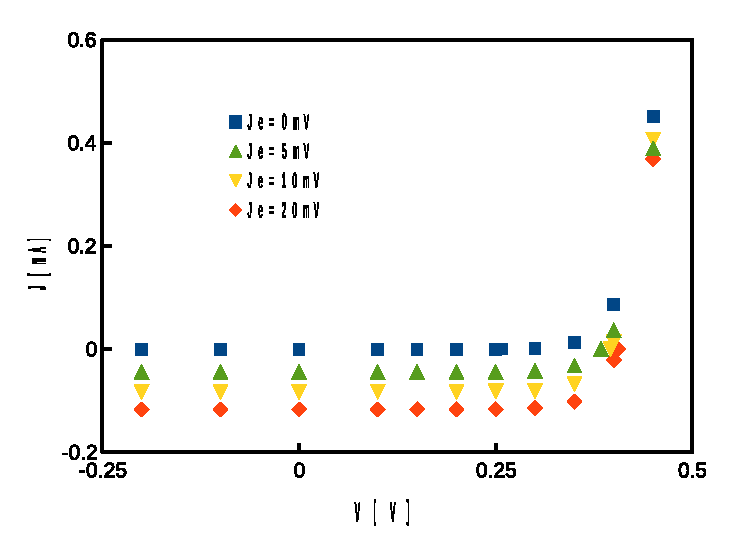
\includegraphics[width=0.8\hsize]{./photodiode.eps}
    \caption{フォトダイオードの電圧電流特性}
     \label{fig:photodiode}
   \end{center}
\end{figure}
\begin{table}[!htbp]
   \begin{center}
  \begin{tabular}{ccc}
    $J_e$ [mA]  & $V_0$ [V] & $J_s$ [mA]\\ \hline
    0 & 0.267 & -0.0004 \\
    5 & 0.384 & -0.0445 \\
    10 & 0.396 & -0.0832 \\
    20 & 0.405 & -0.0117 \\
  \end{tabular}
  \label{tab:Je_Vo_Js}
     \end{center}
       \caption{$J_e$に対する開放電圧$V_0$と短絡電流$J_s$}
\end{table}
\begin{figure}[htbp]
 \begin{minipage}{0.5\hsize}
  \begin{center}
   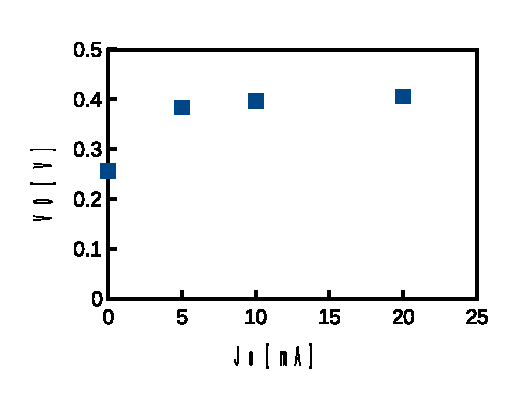
\includegraphics[width=80mm]{Je_V0.eps}
  \end{center}
  \caption{$J_e$と開放電圧$V_0$の関係}
  \label{fig:Je_V0}
 \end{minipage}
 \begin{minipage}{0.5\hsize}
  \begin{center}
   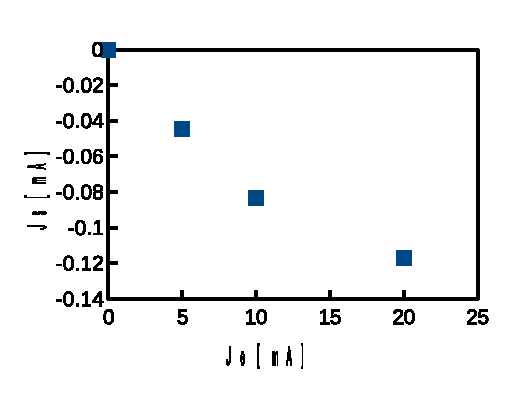
\includegraphics[width=80mm]{Je_Js.eps}
  \end{center}
  \caption{$J_e$と短絡電流$J_s$の関係}
  \label{fig:Je_Js}
 \end{minipage}
\end{figure}

\subsubsection{太陽電池の電圧電流特性}
図\ref{fig:solor_cell}に太陽電池の電圧電流特性をプロットした。図\ref{fig:photodiode}に示したフォトダイオードの電圧電流特性と比較すると、太陽電池は光を照射した際に大きな開放電圧$V_0$と大きな短絡電流$J_s$の絶対値をもつ。
 \begin{figure}[!htbp]
   \begin{center}
    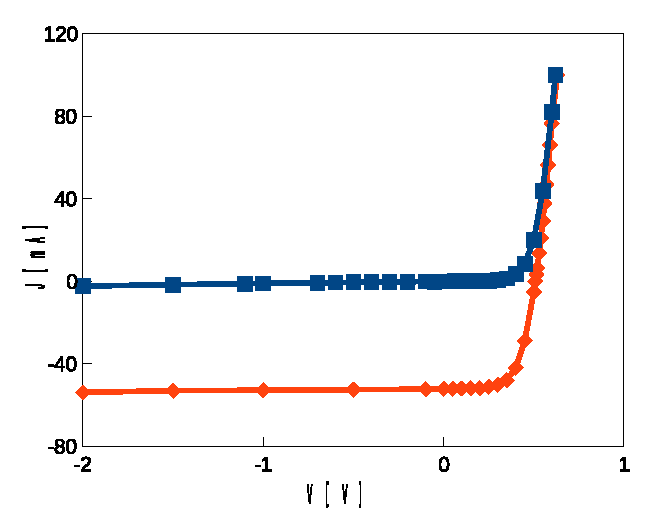
\includegraphics[width=0.6\hsize]{./solor_cell.eps}
    \caption{}
     \label{fig:solor_cell}
   \end{center}
\end{figure}

\subsection{導電率とHall係数の測定}

\subsubsection{室温での導電率とHall係数}
室温での半導体試料の電圧電流特性を図\ref{fig:conductivity_RT}にプロットした。このとき試料に磁場は印加していない。印加した電圧が0Vから0.25Vの間では流れる電流との間に線形性が保たれていることが分かる。
導電率$\sigma$は線形関数の傾きの逆数に比例しその値を$25.69\pm0.10$ [mS/m]と見積もった。試料に63mTの磁場を印加した場合も同様に電気導電率を計算すると、その値は$25.93\pm0.06$ [mS/m]だった。十分に強い磁場を印加すると、電気伝導度はその測定誤差よりも大きな値シフトすることが分かる。

我々の実験条件では磁場による導電率のシフトは十分に小さいため、そのシフトは無視できると今後仮定する。

室温での移動度は0.35[$m^2V^{-1}s^{-1}$]程度と見積もった。

\begin{figure}[!htbp]
   \begin{center}
    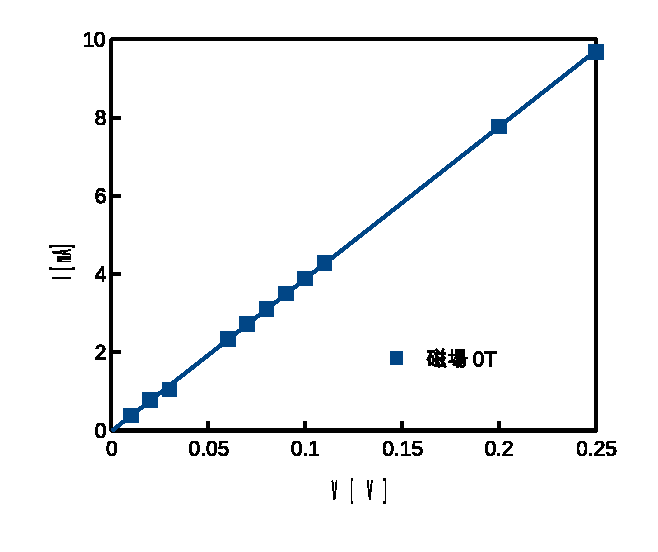
\includegraphics[width=0.5\hsize]{./conductivity_RT.eps}
    \caption{}
     \label{fig:conductivity_RT}
   \end{center}
\end{figure}

\subsubsection{導電率、キャリア密度、移動度の温度依存性}
図\ref{fig:T_sigma}と図\ref{fig:T_R}に、測定した導電率とホール係数の温度特性をそれぞれプロットした。温度が大きくなるにつれて、Hall係数と導電率は小さくなった。
\begin{figure}[htbp]
 \begin{minipage}{0.5\hsize}
   \begin{center}
    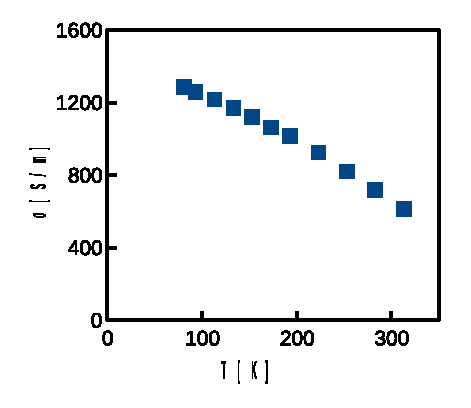
\includegraphics[width=0.8\hsize]{./T_sigma.eps}
    \caption{導電率の温度特性}
     \label{fig:T_sigma}
   \end{center}
 \end{minipage}
 \begin{minipage}{0.5\hsize}
   \begin{center}
    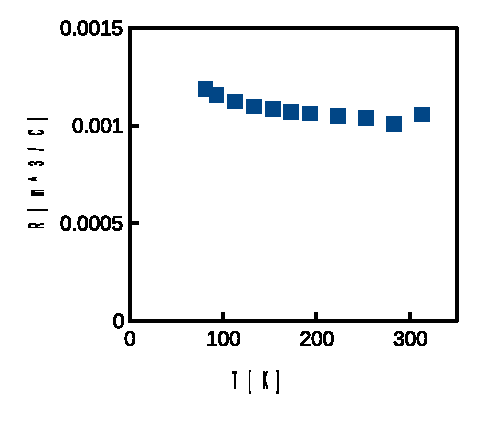
\includegraphics[width=0.8\hsize]{./T_R.eps}
    \caption{ホール係数の温度特性}
     \label{fig:T_R}
   \end{center}
 \end{minipage}
\end{figure}


図\ref{fig:T_n}と図\ref{fig:T_mu}にキャリア密度と移動度をそれぞれプロットした。温度を大きくしてゆくと、キャリア密度は大きくなり移動度は小さくなることがわかる。
特に移動度の温度依存を定量的にさらに分析するために、図\ref{fig:T_mu_log}に移動度を両対数プロットした。以上の温度で$\mu \sim T^{3/2}$がと見て取れる。
\begin{figure}[htbp]
 \begin{minipage}{0.5\hsize}
   \begin{center}
    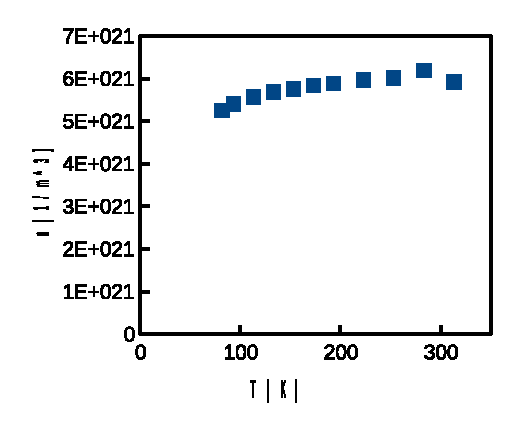
\includegraphics[width=0.8\hsize]{./T_n.eps}
    \caption{キャリア密度の温度特性}
     \label{fig:T_n}
   \end{center}
 \end{minipage}
 \begin{minipage}{0.5\hsize}
   \begin{center}
    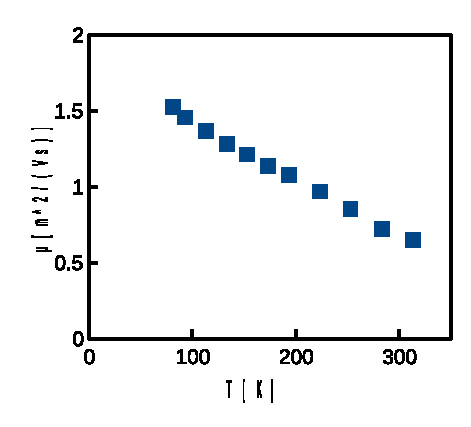
\includegraphics[width=0.8\hsize]{./T_mu.eps}
    \caption{移動度の温度特性}
     \label{fig:T_mu}
   \end{center}
 \end{minipage}
\end{figure}

 \begin{figure}[!htbp]
   \begin{center}
    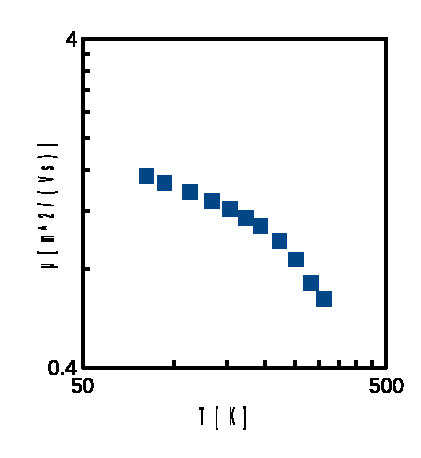
\includegraphics[width=0.4\hsize]{./T_mu_log.eps}
    \caption{移動度の温度特性(両対数プロット)}
     \label{fig:T_mu_log}
   \end{center}
\end{figure}

\section{考察}
\subsection{ダイオード}
\subsubsection{発光ダイオードの発光特性}
発光ダイオードの発光が確認できた最小の印加電圧は、青色で2.6V、緑色で2.7V、赤色で1.5Vだった。この色による発光に必要な電圧の違いは、ギャップエネルギーから定性的に説明できる。ギャップ間遷移が起きるときに発光がおきる波長は印加電圧に依存する。実際、程度である。
\subsubsection{フォトダイオードの電圧電流特性}
フォトダイオードある。

発光ダイオードに流す電流$J_e$を大きくすると開放電圧$V_0$はで説明できる。
さらに$J_e$と短絡電流$J_s$の関係は熱
\subsubsection{太陽電池の電圧電流特性}
フォトダイオードの電圧電流特性と太陽電池の電圧電流特性を比較すると、太陽電池は大きな開放電圧$V_0$と絶対値が大きな短絡電流$J_s$を持つ。この二つの積$V_0J_s$は太陽電池の発電力を意味するため\footnote{正確には図\ref{fig:solor_cell}のように電圧電流特性をプロットしたとき、グラフ上の第3象限の点における$-VJ$が発電力である。}、太陽電池が(フォトダイオードに比べて)効率よく発電できることを意味する。

\subsection{導電率とHall係数の測定}
\subsubsection{室温での導電率とHall係数}
Hall抵抗の値から試料はn型半導体と推定した。
この値はGeの伝導電子の移動度0.36と近い値を持つため、本実験で用いた試料はGeを用いたものと推定する。
\subsubsection{導電率、キャリア濃度、移動度の温度依存性}
イオン化した不純物(-3/2)
フォノンの散乱(-3/2)
キャリア濃度がが上昇するにつれて大きくなることは、から説明できる。

\section{結論}


\end{document}